% Syslab Research Journal Template
% By Patrick White
% September 2019
% version 1.1 - 9/5/2019

% INSTRUCTIONS: Edit the file as appropriate and replace with your journal text. Do NOT edit
%							any section headers or titles, tabling commands, fonts, spacing, sizes, etc.

% -------  Do NOT edit this header
\documentclass[letterpaper,11pt]{article}
\usepackage[paperwidth=8.5in,left=1.0in,right=1.0in,top=1.0in,bottom=1.0in,paperheight=11.0in]{geometry}
\usepackage{palatino}
\usepackage{graphicx}
\def\hrulefill{\leavevmode\leaders\hrule height 20pt\hfill\kern\z@}

% ------------- DO Edit these definitions ---------------------
\def\name{Mikail Khan}
\def\period{5}
\def\journalnum{1}
\def\daterange{9/2/19-9/6/19}
% ------------------ END ---------------------------------

% Do NOT edit this
\begin{document}
	\thispagestyle{empty}
	\begin{flushright}
		{\Large Journal Report \journalnum} \\
		\daterange\\
		\name \\
		Computer Systems Research Lab \\
		Period \period, White
		\end{flushright}
	\hrule height 1pt
% ------------------ END ---------------------------------%	
	
% ------------------- Begin Journal reporting HERE ---------------

% ------ SECTION DAILY LOG -------------------------------------
	\section*{Daily Log}

	\vspace{-0.5em}
        \subsection*{Monday September 2 (Holiday)}
	
                Completed finalizing translational elastic collisions for convex polygons.Also added a way to make immovable objects without just making their mass really high.

		\subsection*{Wednesday September 4}

                I started figuring out how elastic collisions work with translation and rotation. I expected to be able to google a simple equation to implement, but because I have to take into account the possibly numerous contact points between two polygons I ran into lots of problems. Most of the examples online also assume 3D collisions which are inconvenient because I can't cross product 2D vectors without possibly making a new struct for 3D vectors and making all of my 2D vectors 3D vectors with a 0 component. I also realized that the translational part of the collisions is different when taking rotation into account so I started redoing that part. So far, it seems like the direction is correct but energy increases with each collision. 

		\subsection*{Friday September 6}

                I had spent a lot of time last week (first week of school) trying to figure out how to calculate moment of inertia for an arbitrary convex polygon based on its points, but the best solution I came up with was off by around 20\% depending on the number of points you have. I decided to hardcode in moment of inertia for triangles, rectangles, circles etc. so that I can finish the rest of basic mechanics before adding support for arbitrary convex shapes. \\
                I got rotational elastic collisions working a lot better but there are still some weird things happening. Most of the time shapes rotate the correct way after a collision but every so often they seem to rotate in exactly the opposite way. There's also a square that starts rotating super fast as soon as it's touched in the slightest bit. I think both of these should be fixed by checking my vector math.

% ------ SECTION TIMELINE -------------------------------------
	\newpage
	\section*{Timeline}
	\begin{tabular}{|p{1in}|p{2.5in}|p{2.5in}|}
		\hline 
	\textbf{Date} & \textbf{Goal} & \textbf{Met/Details}\\ \hline
		\hline
		August 26th & & Yes \\
		\hline
		September 2nd & & Yes \\
		\hline
                September 6th  & Complete physics helper functions & Mostly, I finished area of a polygon, center of mass, dot product, angle, etc. but decided to leave moment of inertia for later. We also agreed that visual results would be nice. \\
		\hline
                September 13th & Finalize elastic rotational collisisions and persistent contacts & Hopefully the way I'm doing collisisions right now will allow for persistent contacts but I think I'll need to fix some of the logic behind how force works because I was kind of lazy. \\
		\hline
		September 20th& Applying forces to objects besides just during collisions, for example gravity and friction &  \\
		\hline
	\end{tabular}


% ------ SECTION REFLECTION  -------------------------------------
	\section*{Reflection}
        I think I was pretty successful. I didn't quite get rotational collisions to work but I'm optimistic about it. It's fun to watch the shapes float around. I realize that I'll definitely have to make some changes to the core parts of the code, for example right now I'm applying acceleration directly but I think I should add a force field to my collision object structure and I also need to switch from Euler integration to something better.\\
        For some reason my timeline has a goal for Wednesday this week but I think I meant it to be Friday. I'll probably have to work a bit outside of class but I think I'll meet it. I'm looking forwards to finishing up the math/physics parts.
        \begin{figure}
           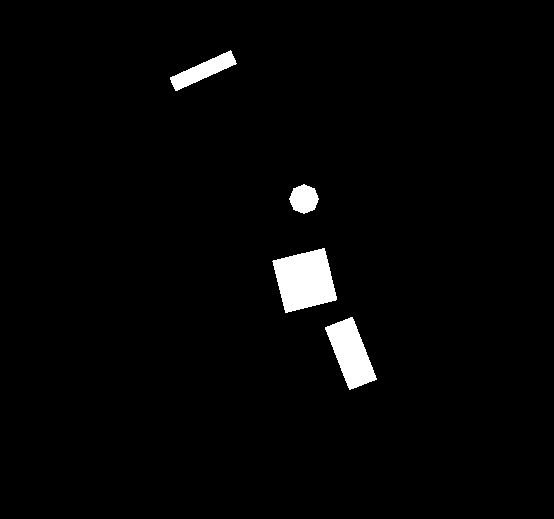
\includegraphics[height=15em]{screen1.png}
           \caption{A boat.}
           \label{fig:boat1}
        \end{figure}
\end{document}
